\sectionbanner{一、单选题}{共10题，每题5分，共50分}

\begin{question}{1}{5}
盒中有红、黄、蓝、绿四种颜色的球，每种颜色各有10个。至少取出多少个球，才能保证无论怎样取，都有一种颜色至少取到4个，并且另有一种不同颜色至少取到3个？
\begin{choices}
  \choice{13}
  \choice{16}
  \choice{17}
  \choice{19}
\end{choices}
\end{question}

\begin{question}{2}{5}
某校科技小组原有60人，其中男生占\(60\%\)。本学期先转入若干名男生，再转出4名女生，此时男生占小组总人数的\(75\%\)。转入的男生有（\quad）人。
\begin{choices}
  \choice{6}
  \choice{12}
  \choice{24}
  \choice{42}
\end{choices}
\end{question}

\begin{question}{3}{5}
四个实数\(a,b,c,d\)满足
\[
  a+b>c+d,\qquad a+c<b+d.
\]
下列关系中一定成立的是哪一个？
\begin{choices}
  \choice{\(a>d\)}
  \choice{\(b>c\)}
  \choice{\(a>c\)}
  \choice{\(b>d\)}
\end{choices}
\end{question}

\begin{question}{4}{5}
如图，在边长为20的正方形\(ABCD\)中剪去一个边长为10的正方形\(DEFG\)。动点\(P\)从点\(B\)出发，以固定速度沿着\(B\to A\to E\to F\to G\to C\)的路线绕多边形运动到停止（不含点\(B\)和点\(C\)），则三角形\(PBC\)的面积\(S\)随着时间\(t\)变化的图象大致为哪个选项？

% Source page: assets/original/page-04.png
\begin{center}
\newcommand{\qivopt}[1]{%
  \begin{tikzpicture}[x=0.155cm,y=0.0066cm,baseline=(current bounding box.center)]
    \draw[-{Stealth[length=1.4mm]}] (0,0)--(8,0) node[below,font=\scriptsize] {\(t\)};
    \draw[-{Stealth[length=1.4mm]}] (0,0)--(0,235) node[left,font=\scriptsize] {\(S\)};
    \draw[red!75!black,thick] #1;
    \node[below left,font=\scriptsize] at (0,0) {\(0\)};
  \end{tikzpicture}%
}
\begin{tabular}{@{}c@{\hspace{3.5mm}}c@{}}
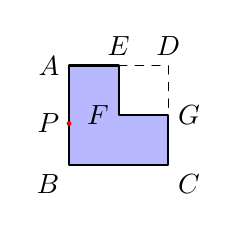
\begin{tikzpicture}[scale=0.42,line cap=round,line join=round,baseline=(current bounding box.center)]
  \fill[blue!28] (0,0)--(0,3)--(1.5,3)--(1.5,1.5)--(3,1.5)--(3,0)--cycle;
  \draw[thick] (0,0)--(0,3)--(1.5,3)--(1.5,1.5)--(3,1.5)--(3,0)--cycle;
  \draw[dashed] (1.5,3)--(3,3)--(3,1.5);
  \fill[red] (0,1.25) circle (2.1pt);
  \node[left]  at (0,3)   {\(A\)};
  \node[above] at (1.5,3) {\(E\)};
  \node[above] at (3,3)   {\(D\)};
  \node[left]  at (1.5,1.5) {\(F\)};
  \node[right] at (3,1.5) {\(G\)};
  \node[below left]  at (0,0) {\(B\)};
  \node[below right] at (3,0) {\(C\)};
  \node[left] at (0,1.25) {\(P\)};
\end{tikzpicture}
&
\setlength{\tabcolsep}{3.2pt}%
\begin{tabular}{@{}ccccc@{}}
  \textcolor{TealDark}{\bfseries A.}\,\qivopt{(0,0)--(2,200)--(3,200)--(4,100)--(6,100)--(7,0)} &
  \textcolor{TealDark}{\bfseries B.}\,\qivopt{(0,200)--(3,200)--(3,100)--(6,100)--(6,0)} &
  \textcolor{TealDark}{\bfseries C.}\,\qivopt{(0,0)--(3,200)--(4,100)--(6,100)--(7,0)} &
  \textcolor{TealDark}{\bfseries D.}\,\qivopt{(0,0)--(2,200)--(3,200)--(4,50)--(6,50)--(7,0)} &
  \textcolor{TealDark}{\bfseries E.}\,\qivopt{(0,0)--(2,200)--(5,200)--(7,0)}
\end{tabular}
\end{tabular}
\end{center}
\end{question}

\begin{question}{5}{5}
乘积 \(20\times21\times22\times23\times24\times25\) 的末尾共有（\quad）个连续的0。
\begin{choices}
  \choice{2}
  \choice{3}
  \choice{4}
  \choice{5}
\end{choices}
\end{question}

\begin{question}{6}{5}
三个连续正整数的乘积恰好等于它们之和的33倍。这三个数中最大的一个是（\quad）。
\begin{choices}
  \choice{9}
  \choice{10}
  \choice{11}
  \choice{12}
\end{choices}
\end{question}

\begin{question}{7}{5}
如图，8个半径都是\(5\text{ cm}\)的圆排列在一起，\(AB\)、\(DC\)是直径，则梯形\(FBCE\)的面积是多少平方厘米？

% Source page: assets/original/page-07.png
\begin{center}
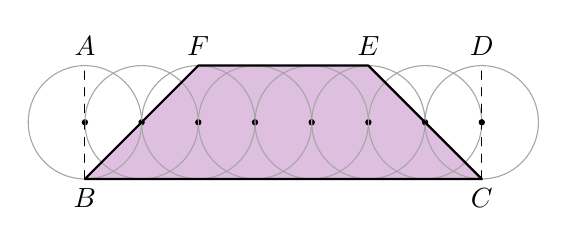
\begin{tikzpicture}[scale=0.72,line cap=round,line join=round]
  \fill[violet!25] (0,-1)--(2,1)--(5,1)--(7,-1)--cycle;
  \foreach \x in {0,...,7}{
    \draw[gray!70] (\x,0) circle (1);
    \fill (\x,0) circle (1.6pt);
  }
  \draw[thick] (0,-1)--(2,1)--(5,1)--(7,-1)--cycle;
  \draw[dashed] (0,-1)--(0,1);
  \draw[dashed] (7,-1)--(7,1);
  \node[above] at (0,1) {\(A\)};
  \node[below] at (0,-1) {\(B\)};
  \node[above] at (2,1) {\(F\)};
  \node[above] at (5,1) {\(E\)};
  \node[above] at (7,1) {\(D\)};
  \node[below] at (7,-1) {\(C\)};
\end{tikzpicture}
\end{center}

\begin{choices}
  \choice{250}
  \choice{300}
  \choice{240}
  \choice{360}
  \choice{320}
\end{choices}
\end{question}

\begin{question}{8}{5}
甲组有24名学生，平均分为85分；乙组有21名学生，平均分为79分。现将甲组中的\(k\)名学生调入乙组，这\(k\)名学生原来在甲组的平均分记为\(s\)。调动后，乙组的平均分恰好为81分，且这\(k\)名学生的平均分\(s\)比甲组余下学生的平均分恰高4分。则\(k\)的值为（\quad）。
\begin{choices}
  \choice{4}
  \choice{5}
  \choice{6}
  \choice{7}
\end{choices}
\end{question}

\enlargethispage{16mm}
\begin{question}{9}{5}
古镇广场上的喷泉与塔楼上的时钟相连：只要时钟的指针（时针或分针）中至少有一根位于数字3和4之间，或者位于8和9之间，喷泉就会运作。请问在一昼夜（24小时）内，这个喷泉运作的总时间是多少？

% Source page: assets/original/page-09.png
{\centering
\vspace{-1mm}
\begin{tikzpicture}[scale=0.44,line cap=round]
  \fill[blue!22] (0,0)--(2.15,0) arc[start angle=0,end angle=-30,radius=2.15]--cycle;
  \fill[blue!22] (0,0)--({2.15*cos(-150)},{2.15*sin(-150)})
    arc[start angle=-150,end angle=-180,radius=2.15]--cycle;
  \draw[very thick] (0,0) circle (2.15);
  \foreach \n in {1,...,12}{
    \pgfmathsetmacro{\ang}{90-30*\n}
    \node at ({1.78*cos(\ang)},{1.78*sin(\ang)}) {\small \n};
  }
  \draw[very thick,-{Stealth[length=2.2mm]}] (0,0)--({1.55*cos(120)},{1.55*sin(120)});
  \draw[very thick,-{Stealth[length=2.2mm]}] (0,0)--({1.42*cos(-80)},{1.42*sin(-80)});
  \fill (0,0) circle (2pt);
\end{tikzpicture}\par}

\begin{choices}
  \choice{11小时40分钟}
  \choice{9小时30分钟}
  \choice{7小时20分钟}
  \choice{5小时40分钟}
  \choice{4小时}
\end{choices}
\end{question}

\begin{question}{10}{5}
对正整数\(n\)，定义
\[
  F(n)=|n-1|+2|n-2|+3|n-3|+\cdots+17|n-17|.
\]
则\(F(n)\)的最小值为（\quad）。
\begin{choices}
  \choice{542}
  \choice{521}
  \choice{524}
  \choice{585}
\end{choices}
\end{question}

\sectionbanner{二、填空题}{共5题，每题6分，共30分}

\begin{question}{11}{6}
正整数\(a,b\)满足
\[
  \frac{3}{8}<\frac{a}{b}<\frac{2}{5}.
\]
则\(b\)的最小值为\answerline
\end{question}

\begin{question}{12}{6}
甲从\(P\)地出发，沿同一路线向\(Q\)地行进，速度为每分钟90米。半分钟后，乙也从\(P\)地出发前往\(Q\)地，速度为每分钟60米。甲到达\(Q\)地后停留1分钟，再立即原路返回；返回时速度仍为每分钟90米；乙始终向\(Q\)地行进。乙出发后，两人第一次相遇的地点距\(P\)地270米。\(P\)、\(Q\)两地相距\answerline 米。
\end{question}

\begin{question}{13}{6}
如图，长方形\(ABCD\)中有4个周长均为18的小长方形。现将长方形\(EFGH\)放在\(ABCD\)内，与4个小长方形正好重叠出4个涂色小长方形。已知\(AB=12\)，\(BC=14\)，4个涂色小长方形的周长和是24，则长方形\(EFGH\)的周长是多少？

% Source page: assets/original/page-13.png
\begin{center}
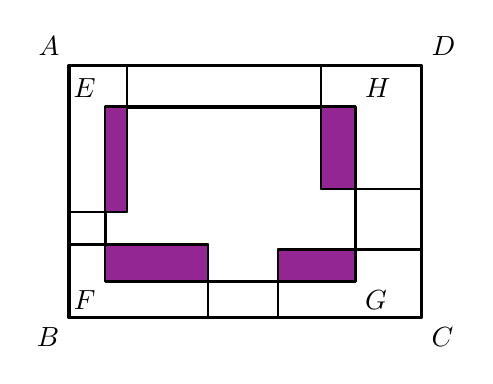
\begin{tikzpicture}[scale=0.64,line cap=round,line join=round]
  \draw[very thick] (0,0) rectangle (7,5);
  % Four corner rectangles
  \draw[thick] (0,2.1) rectangle (1.15,5);
  \draw[thick] (5.0,2.55) rectangle (7,5);
  \draw[thick] (0,0) rectangle (2.75,1.45);
  \draw[thick] (4.15,0) rectangle (7,1.35);
  % Inner rectangle EFGH
  \draw[very thick] (0.72,0.72) rectangle (5.68,4.18);
  % Four overlap rectangles
  \fill[violet!85] (0.72,2.1) rectangle (1.15,4.18);
  \fill[violet!85] (5.0,2.55) rectangle (5.68,4.18);
  \fill[violet!85] (0.72,0.72) rectangle (2.75,1.45);
  \fill[violet!85] (4.15,0.72) rectangle (5.68,1.35);
  \draw[thick] (0.72,2.1) rectangle (1.15,4.18);
  \draw[thick] (5.0,2.55) rectangle (5.68,4.18);
  \draw[thick] (0.72,0.72) rectangle (2.75,1.45);
  \draw[thick] (4.15,0.72) rectangle (5.68,1.35);
  \node[above left]  at (0,5) {\(A\)};
  \node[below left]  at (0,0) {\(B\)};
  \node[below right] at (7,0) {\(C\)};
  \node[above right] at (7,5) {\(D\)};
  \node[above left]  at (0.72,4.18) {\(E\)};
  \node[below left]  at (0.72,0.72) {\(F\)};
  \node[below right] at (5.68,0.72) {\(G\)};
  \node[above right] at (5.68,4.18) {\(H\)};
\end{tikzpicture}
\end{center}

\answerline
\end{question}

\begin{question}{14}{6}
求最小的正整数\(M\)，使得能从\(0,1,\ldots,M\)中选出5个整数，并且这5个数两两作“大数减小数”所得的10个正差互不相同。
\[
  M=\answerline
\]
\end{question}

\begin{question}{15}{6}
从1至100中选择12个不同的数字填入圆圈中，使得每个数字要么是其相邻两个数字的最大公因数，要么是它们的最小公倍数。假设已经填入了5个数字（如图所示），求\(x\)处可以填入的所有不同数字之和。

% Source page: assets/original/page-15.png
{\centering
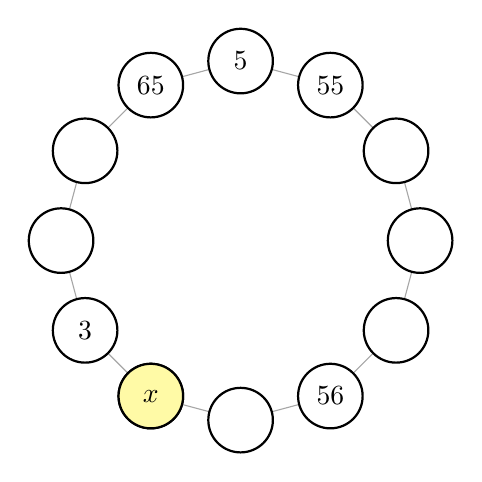
\begin{tikzpicture}
  \foreach \i in {1,...,12}{
    \pgfmathsetmacro{\ang}{120-30*\i}
    \coordinate (c\i) at (\ang:2.28cm);
  }
  \foreach \i in {1,...,12}{
    \pgfmathtruncatemacro{\j}{mod(\i,12)+1}
    \draw[gray!70] (c\i)--(c\j);
  }
  \foreach \i in {1,...,12}{
    \node[draw,thick,circle,minimum size=8.2mm,inner sep=0pt,fill=white] at (c\i) {};
  }
  \node[draw,thick,circle,minimum size=8.2mm,inner sep=0pt,fill=yellow!35] at (c8) {\(x\)};
  \node at (c1) {\(5\)};
  \node at (c2) {\(55\)};
  \node at (c6) {\(56\)};
  \node at (c9) {\(3\)};
  \node at (c12) {\(65\)};
\end{tikzpicture}\par}

\answerline
\end{question}

\sectionbanner{三、多选题}{共4题，每题7分，共28分}

\begin{question}{16}{7}
袋中有3个红球、4个蓝球和2个黄球，9个球除颜色外均可区分。先随机同时取出2个球且不放回，再随机取出第3个球。已知第一次取出的2个球中至少有1个黄球。下列说法中正确的是哪些？
\begin{multichoices}
  \choice{第一次恰好取到1个黄球的条件概率为\(\frac{14}{15}\)}
  \choice{第3个球是黄球的条件概率为\(\frac{2}{15}\)}
  \choice{取出的3个球中恰有1个黄球的条件概率为\(\frac45\)}
  \choice{取出的3个球都不是红球的条件概率为\(\frac13\)}
\end{multichoices}
\end{question}

\begin{question}{17}{7}
有7名学生。现列出若干个互不相同的两人小组，组成一份小组清单，要求清单中任意两个小组都有1名共同学生。只要所列两人小组的集合不同，就视为不同清单。下列说法中正确的是哪些？
\begin{multichoices}
  \choice{任意一份符合要求的清单最多含有6个小组}
  \choice{若一份符合要求的清单至少含有4个小组，则必有一名学生出现在清单的所有小组中}
  \choice{恰有7种符合要求的清单含有6个小组}
  \choice{恰有35种符合要求的清单满足：任取一个尚未列入清单的两人小组，将其加入后，都会使新清单不再满足上述要求}
\end{multichoices}
\end{question}

\begin{question}{18}{7}
从有序数对\((1,1)\)出发，每一步可以选择下列一种操作：
\[
  (x,y)\longrightarrow(x+y,y),
  \qquad\text{或}\qquad
  (x,y)\longrightarrow(x,x+y).
\]
下列说法中正确的是哪些？
\begin{multichoices}
  \choice{\((8,19)\)可以恰好经过6步到达}
  \choice{除起点外，每个可到达的数对都有且只有一个可到达的前驱数对，从该前驱经过一步操作可以得到它}
  \choice{除起点\((1,1)\)外，任何可到达的数对的两个坐标都不相等}
  \choice{\((7,23)\)可以恰好经过6步到达}
\end{multichoices}
\end{question}

\begin{question}{19}{7}
有9枚外观相同的硬币，其中恰有1枚比其余8枚重。现用无砝码天平称量；每次称量时两盘放相同枚数的硬币，天平结果只有“左盘重”“右盘重”“平衡”三种。最多称量2次，第二次可以根据第一次的结果安排。下列说法中正确的是哪些？
\begin{multichoices}
  \choice{任意能保证找出重硬币的方案，第一次称量时两盘必须各放3枚硬币}
  \choice{第一次把3枚硬币对3枚硬币称量；若平衡，第二次在未称量的3枚中取1枚对1枚；若不平衡，第二次在较重盘的3枚中取1枚对1枚；这一方案一定能找出重硬币}
  \choice{即使第二次称量的摆放方案必须在第一次结果出来前固定，仍存在保证2次找出重硬币的方案}
  \choice{若有10枚硬币仍最多称量2次，第一次把3枚对3枚称量且恰好平衡，则第二次仍一定能找出重硬币}
\end{multichoices}
\end{question}

\Needspace{11cm}
\sectionbanner{四、综合题}{共3题，每题14分，共42分}

\begin{question}{20}{14}
现有大小相同的正方形卡片，每张卡片上分别写着从1到300的一个数字。将这300张卡片按照从小到大的顺序排列，在1号卡片的右边放2号卡片，在它正下方放3号卡片，依此类推，顺时针呈螺旋状排列。

% Source page: assets/original/page-20.png
\begin{center}
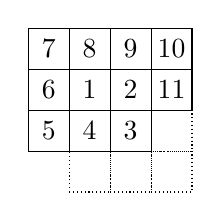
\begin{tikzpicture}[scale=0.52]
  \foreach \x in {0,1,2}{
    \foreach \y in {0,1,2}{
      \draw (\x,\y) rectangle ++(1,1);
    }
  }
  \draw (3,1) rectangle ++(1,1);
  \draw (3,2) rectangle ++(1,1);
  \draw[densely dotted] (3,0) rectangle ++(1,1);
  \foreach \x in {1,2,3}{
    \draw[densely dotted] (\x,-1) rectangle ++(1,1);
  }
  \node at (0.5,2.5) {\(7\)};
  \node at (1.5,2.5) {\(8\)};
  \node at (2.5,2.5) {\(9\)};
  \node at (3.5,2.5) {\(10\)};
  \node at (0.5,1.5) {\(6\)};
  \node at (1.5,1.5) {\(1\)};
  \node at (2.5,1.5) {\(2\)};
  \node at (3.5,1.5) {\(11\)};
  \node at (0.5,0.5) {\(5\)};
  \node at (1.5,0.5) {\(4\)};
  \node at (2.5,0.5) {\(3\)};
\end{tikzpicture}
\end{center}

\subquestion{4}{当排完25张卡片时，与25号卡片位于同一竖列，包含25号卡片在内，共有多少张？}
\answerspace

\subquestion{5}{按照顺序继续排列卡片时，100号卡片周围的卡片分布会是怎样的？请写出表格中“好”字处（即左下角）所对应的数字。}

% Source page: assets/original/page-21.png
\begin{center}
\begingroup
\setlength{\tabcolsep}{0.7em}
\renewcommand{\arraystretch}{1.25}
\begin{tabular}{|c|c|c|}
  \hline
  \phantom{100} & \phantom{100} & \phantom{100} \\ \hline
  & \(100\) & \\ \hline
  好 & & \\ \hline
\end{tabular}
\endgroup
\end{center}
\answerspace

\subquestion{5}{当排完所有300张卡片时，在与300号卡片位于同一横排的所有卡片中，写出其中最小的数字。}
\answerspace
\end{question}

\begin{question}{21}{14}
将小于1的最简分数按照如下规则排列，并将分母相同的分数分在同一个组中。最简分数是指不能再进行约分的分数。

% Source page: assets/original/page-23.png
\[
\begin{array}{c|cc|cc|cccc|cc|c}
 \dfrac12
 & \dfrac13 & \dfrac23
 & \dfrac14 & \dfrac34
 & \dfrac15 & \dfrac25 & \dfrac35 & \dfrac45
 & \dfrac16 & \dfrac56
 & \cdots\\[2.4ex]
 \text{第1组}
 & \multicolumn{2}{c|}{\text{第2组}}
 & \multicolumn{2}{c|}{\text{第3组}}
 & \multicolumn{4}{c|}{\text{第4组}}
 & \multicolumn{2}{c|}{\text{第5组}}
 & 
\end{array}
\]

\subquestion{4}{第71组中排列了多少个分数？}
\answerspace

\subquestion{5}{到第420组为止，分子为3的分数共有多少个？}
\answerspace

\subquestion{5}{对于从第20组到第30组的所有分数，将它们的分子全部相乘。这个乘积能被5整除多少次？（“能被整除”是指商为整数且余数为0。）}
\answerspace
\end{question}

\begin{question}{22}{14}
有三个厚度相同的圆盘\(A\)、\(B\)、\(C\)，它们的直径分别是\(20\text{ cm}\)、\(30\text{ cm}\)、\(40\text{ cm}\)。每个圆盘的圆周上都有将其24等分的刻度，如图1所示，顺着刻度按顺时针方向依次标有数字1到24。将这些圆盘如图2所示相切放置，固定它们的中心，当顺时针旋转圆盘\(A\)时，\(B\)会逆时针旋转，\(C\)则会顺时针旋转，且它们之间转动时不会发生滑动。此外，可以在圆盘的侧面（边缘）涂上颜料，通过旋转圆盘，相切接触的地方就会把颜色印到相邻圆盘的侧面上。

% Source page: assets/original/page-26.png, Figure 1
\begin{center}
\begin{tikzpicture}[scale=0.72,line cap=round,line join=round,baseline=(figone.base)]
  \fill[gray!18] (-2,0)--(-2,-0.65) arc[start angle=180,end angle=360,x radius=2,y radius=0.55]
    --(2,0) arc[start angle=360,end angle=180,x radius=2,y radius=0.65]--cycle;
  \draw[thick] (0,0) ellipse (2 and 0.65);
  \draw[thick] (-2,0)--(-2,-0.65);
  \draw[thick] (2,0)--(2,-0.65);
  \draw[thick] (-2,-0.65) arc[start angle=180,end angle=360,x radius=2,y radius=0.55];
  \foreach \n in {1,...,24}{
    \pgfmathsetmacro{\ang}{450-15*\n}
    \draw[gray!70] ({1.92*cos(\ang)},{0.62*sin(\ang)})
      --({2.03*cos(\ang)},{0.66*sin(\ang)});
    \node[scale=0.43] at ({2.23*cos(\ang)},{0.86*sin(\ang)}) {\n};
  }
  \foreach \ang in {195,210,...,345}{
    \draw[gray!65] ({2*cos(\ang)},{0.65*sin(\ang)})
      --({2*cos(\ang)},{0.65*sin(\ang)-0.58});
  }
  \fill (0,0) circle (2pt);
  \node (figone) at (0,1.48) {图1};
  \node[right] at (2.15,-0.42) {侧面};
\end{tikzpicture}
\hspace{1.2em}
% Source page: assets/original/page-26.png, Figure 2
\begin{tikzpicture}[scale=0.74,line cap=round,line join=round,baseline=(figtwo.base),
  arr/.style={-{Stealth[length=2.4mm,width=1.9mm]},line width=1.15pt}]
  \coordinate (A) at (0,0);
  \coordinate (B) at (2.5,0);
  \coordinate (C) at (6.0,0);
  \draw[thick,fill=gray!12] (A) circle (1);
  \draw[thick,fill=gray!12] (B) circle (1.5);
  \draw[thick,fill=gray!12] (C) circle (2);
  % +1mm on the printed page: 1mm / 0.74cm per unit
  \foreach \p/\rin in {A/0.715,B/1.235,C/1.715}{
    \fill (\p) circle (1.5pt);
    \node[font=\scriptsize] at ($(\p)+(0,\rin)$) {24};
    \node[font=\scriptsize] at ($(\p)+(\rin,0)$) {6};
    \node[font=\scriptsize] at ($(\p)+(0,-\rin)$) {12};
    \node[font=\scriptsize] at ($(\p)+(-\rin,0)$) {18};
  }
  \begin{scope}[shift=(A)]
    \draw[arr] (135:1.11) arc[start angle=135,delta angle=-85,radius=1.11];
  \end{scope}
  \begin{scope}[shift=(B)]
    \draw[arr] (-135:1.61) arc[start angle=-135,delta angle=85,radius=1.61];
  \end{scope}
  \begin{scope}[shift=(C)]
    \draw[arr] (130:2.11) arc[start angle=130,delta angle=-80,radius=2.11];
  \end{scope}
  \node at (0,-2.65) {\(A\)};
  \node at (2.5,-2.65) {\(B\)};
  \node at (6.0,-2.65) {\(C\)};
  \node (figtwo) at (3.0,2.82) {图2};
\end{tikzpicture}
\end{center}

\subquestion{4}{一开始不涂颜料，将\(A\)、\(B\)、\(C\)三个圆盘都按“24”号刻度朝向正上方的位置放置好。接着，将\(A\)顺时针旋转90度，使得其“18”号刻度来到正上方。此时，求圆盘\(C\)正上方的数字。}
\answerspace

\subquestion{5}{这一次，在圆盘\(A\)的整个侧面都涂满颜料。然后，如图2所示将\(A\)、\(B\)、\(C\)再次都按“24”号刻度朝向正上方放置好，接着开始旋转\(A\)，直到圆盘\(C\)的侧面全部被印上颜料为止。请问，恰好在圆盘\(C\)的整个侧面都被印满颜料的那一刻，圆盘\(C\)正上方的数字是多少？}
\answerspace

\subquestion{5}{将圆盘侧面沾上的颜色全部擦除干净后，在圆盘\(A\)侧面从刻度“18”开始顺时针到刻度“6”的这部分区间涂上颜料。然后，如图2所示将\(A\)、\(B\)、\(C\)再次都按“24”号刻度朝向正上方放置好，接着开始旋转\(A\)，直到圆盘\(C\)的侧面全部被印上颜料为止。请问，恰好在圆盘\(C\)的整个侧面都被印满颜料的那一刻，圆盘\(C\)正上方的数字是多少？}
\answerspace
\end{question}
